\section{Simulation Results and Metrics}
\label{simulation}

Verifying the correct function of a schedule generator can be a daunting task.  Below we describe our testing tool, give an example of partial model debugging, and show performance metrics.

\subsection{Test Generation}

Finding a large variety of realistic scheduling problem instances of significant size presented a testing challenge for our scheduler-building effort.  We created a simulator that builds random networks, populates the processing nodes with tasks, and then creates a random network-compatible task dependency graph representing messages.  The problem generator parameters are shown below:

\begin{itemize}
\item {\bf nodes} -- Number of processing nodes in the system.
\item {\bf networks} -- Number of networks (buses) in the system.
\item {\bf nets-per-node} -- Max networks connected to a node.
\item {\bf max-tasks} -- Max tasks running on a node.
\item {\bf period} -- Fundamental period of tasks(secs).  Actual period of a task is either the fundamental period, one half, or one quarter of the fundamental period.
\item {\bf msg-prob} -- Probability of creating a message between two tasks.  This roughly corresponds to the probability parameter for an Erdos-Renyi random graph on each subset of tasks attached to the same network.
\item {\bf min-msg, max-msg} -- Minimum/maximum message length (bytes).  Message lengths are randomly chosen from this interval (uniform distribution).
\item {\bf min-util, max-util} -- Minimum/maximum task utilization (drawn uniformly from (0.0,1.0)).  This parameter controls the chosen task deadline, which is a fraction of the period.
\item {\bf sys-res} -- System resolution (in seconds).
\end{itemize}

During generation no effort is made to ensure that the network topology is connected, but randomly adding edges between nodes in different graph components can easily ensure connectivity if desired.  The tester uses the Boost graph library\cite{tools:bgl} for graph structure manipulation.

\subsection{Test Cases}

For the specification given in listing \ref{schedspec}, ESched returned the following schedule:

\begin{framed}
\lstset{basicstyle=\small,frame=none,label=schedrslt,caption=Sample schedule.}

\begin{lstlisting}
Hyperperiod 40 ms

B12:
B12/M1_0 19.932
B12/M1_1 30.092

B23:
B23/M3_0 19.958
B23/M2_0 19.99
B23/M3_1 30.018

P1:
P1/T2_0 4.986
P1/T1_0 9.934
P1/T2_1 14.986
P1/T2_2 24.986
P1/T1_1 29.934
P1/T2_3 34.986

P2:
P2/T2_0 0.044
P2/T1_0 9.994
P2/T2_1 10.044
P2/T2_2 20.044
P2/T1_1 29.994
P2/T2_3 30.044

P3:
P3/T2_0 9.984
P3/T1_0 19.994
P3/T2_1 29.984

\end{lstlisting}
\end{framed}

The schedule lists the release (transfer) times (in milliseconds) for each instance of the tasks and messages given in the spec.  Each start time is a multiple of the specified resolution.  For a partial model, we give an option to the scheduler as follows:

\begin{framed}
\lstset{basicstyle=\small,frame=none,label=schedrslt2,caption=Sample schedule.}

\begin{lstlisting}
ESched.exe -f test.scs -o test.rslt 
  -d P2 -d P1

P1:
P1/T2_0: 4.992
P1/T1_0: 9.994
P1/T2_1: 14.992
P1/T2_2: 24.992
P1/T1_1: 29.994
P1/T2_3: 34.992

P2:
P2/T2_0: 0.044
P2/T1_0: 9.994
P2/T2_1: 10.044
P2/T2_2: 20.044
P2/T1_1: 29.994
P2/T2_3: 30.044
\end{lstlisting}
\end{framed}

Listing \ref{schedrslt2} shows the schedule only for the tasks on processors P1 and P2, without their message dependencies.  This type of partial model is useful for isolating a single processor with an infeasible task set, for example.  Observe that this is only useful for checking feasibility -- the calculated release times are not necessarily the same as for the global problem.

\subsection{Metrics}

Fig. 5 shows execution time for a number of `fast' test cases.  Many feasible scheduling problems resolve very quickly with our current heuristics.  A very few infeasible problems resolve quickly as well, while some problems from both classes enter a long search phase.  The boundaries of these cases are not well-characterized.  ESched still neeeds rigorous testing and tuning, so these results must be considered preliminary. Maximum memory utilization for long-running problems appears in Fig. 6.  The Gecode solver appears to do an excellent job of managing memory consumption, as memory usage levels remain fairly stable during long searches.  The results shown here are given for randomly-generated problems of different sizes.  Generation parameters were chosen only to keep the problems on the ``edge" of solvability, where a fair number of test cases would be quickly solvable, and the others would be more difficult.  The resolution parameter can seriously affect the size of the search space, so it must be chosen with care.  Ideally it should represent a fundamental scheduling quantum in the physical system, but it may need to be reduced if the searches take too long.

\begin{figure}[ht]
		%[height=50mm,width=50mm]
	  \label{fig:exectime}
		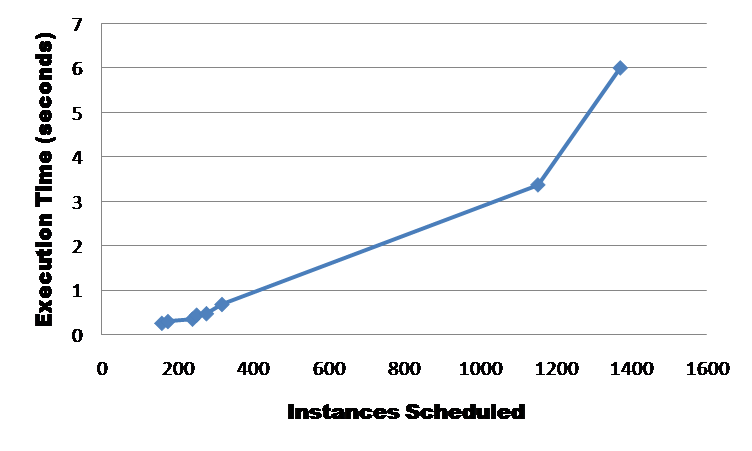
\includegraphics[scale=.7]{figures/exectime.png}
		\centering
		\caption{Execution time for feasible instances.}
\end{figure}

\begin{figure}[ht]
		%[height=50mm,width=50mm]
		\label{fig:memusage}
		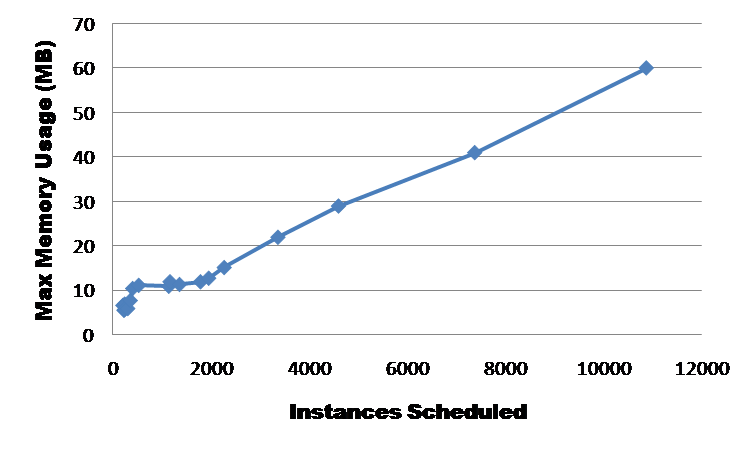
\includegraphics[scale=.7]{figures/memusage.png}
		\centering
		\caption{Maximum memory consumption vs. problem instance size.}
\end{figure}
